%************************************************
\chapter{Discussion}\label{ch:Discussion} 
%************************************************
\section{Suitability of SID}
The Shared Imbalance Detection (SID) tool, written in Python and utilising a MS-SQL database can scan a directory, parsing feature extraction files and by applying a Z score algorithm can detect regions of shared CNV from manually created true positive cases with a sensitivity of 100\% in a timely fashion.


\section{Z score threshold to define a probe as abnormal}
Analysis of the training cases identified suitable thresholds to be applied however the training cases were not truly representative of routine feature extraction files.
\paragraph*{}
Analysis of the test cases suggest that using a threshold of between 3.55 and 4 to define a probe as abnormal would detect all shared copy number variation without any false positive calls. 

\paragraph*{}
Applying the lower threshold to prospective arrays resulted in calls in 1 in 9 cases. However some cases contained a large number of calls, which would increase the analysis burden. Further investigation into why some arrays contain a much higher number of calls and a strategy to predict and manage these arrays may be required.

\section{The number of probes within true positive calls}
The proportion of probes called as abnormal within the true positive calls was not assessed in detail as each call serves as a flag to prompt further investigation by the analyst who would further describe the exact shared CNV.
\paragraph*{}
Whilst the entire CNV may not be called, the calls may be spread out across the CNV, giving an indication of the shared CNV.
\paragraph*{}
Why so little of the large chromosome 22 deletion was not called should be investigated further.

\section{Combining overlapping trios of abnormal probes}
A strategy has been created to combine trios of shared abnormal probes in line with existing analysis protocols.

\section{Benign CNV}
It is expected that hybridisation partners would share one or more of the many known, common benign CNV regions. SID would correctly identify these regions as abnormal, however the above analysis would classify these calls as false positives. It may be worth excluding these regions from future specificity and sensitivity calculations
\paragraph*{}
Should SID be adopted by the clinical service stakeholders should be consulted to determine if calls within known benign CNV regions should be filtered out, or  if the experience of clinical scientists would make analysis of common calls trivial.


\section{Calls smaller than 5 probes}
The vast majority of false positive calls in the test set and prospective arrays contain less than 5 probes (Table \ref{tab:prosepectivecalls} and Figure \ref{fig:testcasesprobecount}). 
\paragraph*{}
The average signal intensity of probes within a true positive call is higher than that of a false positive call (Figure \ref{fig:testcasesaverageconfidenceZscore}) so a secondary analysis could be applied to further reduce false positive calls. 

\section{Different thresholds for gain or loss}
The proportional signal intensity change between diploid and triploid and diploid and monosomy is the same ($\pm$50\%). Therefore the Z score would be the same for monosomy and trisomy. 
\paragraph*{}
Similar numbers of false positive gains and losses suggest using the same threshold for losses and gains does not introduce bias however should further work identify a lack of sensitivity for either gain or loss separate thresholds could be applied.

\section{Alternative approaches to consecutive probes analysis}
\subsection{Larger sliding windows}
The Z score algorithm implemented differs to that suggested by Agilent who suggest a sliding window and the proportion of probes outside a threshold used to define a region as abnormal \cite{agilent_technologies_agilent_2011}.
\paragraph*{}
This approach may result in a call which does not meet the specification (Figure \ref{fig:incorrectcallandalternatecomb}a).
\paragraph*{}
The consecutive probe approach applied within SID is designed to match the routine analysis approach however a sliding window approach would prevent aberrations such as those in Figure \ref{fig:incorrectcallandalternatecomb}b being missed.

\begin{figure}[h]
\centering
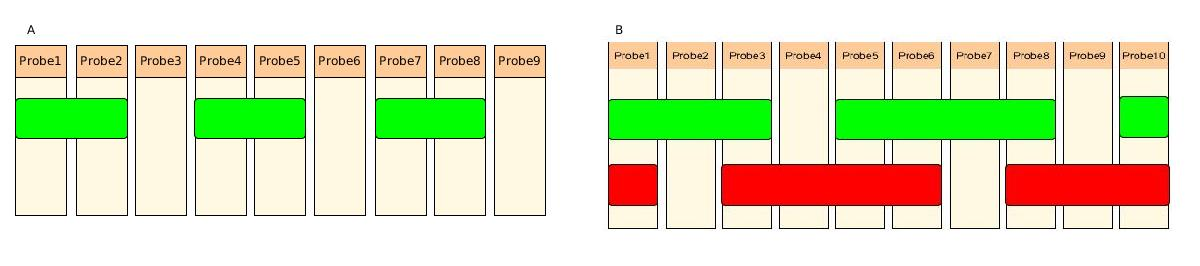
\includegraphics[width=1\linewidth]{./Figures/incorrectcallandalternatecomb}
\caption[Classifying overlapping shared CNV]{Classifying overlapping shared CNV. a. Using a sliding window approach and measuring the proportion of probes outside a threshold may result in calls which do not meet the functional specification of three consecutive probes.\\
b. The existing algorithm may miss clearly overlapping CNV where three consecutive abnormal probes are not shared}
\label{fig:incorrectcallandalternatecomb}
\end{figure}

\subsection{Sliding window - Regions of interest}
A variation of the sliding window approach was investigated, using defined regions of interest (every CNV which has been reported more than twice) as a window. The same Z score analysis was performed and the proportion of abnormal probes within the region used to determine if a region is abnormal or not.
\paragraph*{}
Despite this approach being targeted to known clinically relevant CNV and the potential to expand the list of regions this approach is more limited than the consecutive probe approach so was not pursued.

\section{Further work}
\subsection{Sex chromosomes}
Further work is required to include sex chromosomes in the analysis. The gender of the sample affects the signal intensities of probes on the sex chromosomes. 
\paragraph*{}
To identify CNV on the sex chromosomes a gender specific reference range is required. The average signal intensity across non pseudoautosomal regions of the X and Y chromosomes could determine gender and therefore which reference range should be applied.
\subsection{Sample type}
This project has only assessed postnatal blood samples. The array service also processes prenatal, solid tissue and \ac{PGD} samples, which have variable resolution and performance due to the quality of the sample. 
\paragraph*{}
Differing analysis strategies and Z score thresholds would be required for each sample type in line with existing analysis approaches in addition to a method for specifying the sample type of each array.
\subsection{What happens when shared CNV is detected?}
Once shared CNV is detected further investigation is required. The level of investigation required would dictate the acceptable levels of specificity of SID. If a thorough investigation is required the time and cost incurred would negate any savings made by replacing phenotype mismatching with SID.
\paragraph*{}
The signal intensities can be examined within the analysis software which would confirm or deny the presence of CNV in line with the current approach to identify if an call is a duplication in one hybridisation partner or a deletion in the other. However having more than 50 calls on a single array would make this approach unfeasible.
\paragraph*{}
Another potential approach is EvE, a tool which allows post hoc hybridisation of samples. Each sample could be independently analysed against another sample, such as a reference control, to see if CNV is present. 
\paragraph*{}
EvE takes about one minute to run and the analysis could be performed in less than 10 minutes. However should this be required routinely any time savings would be diminished.
EvE has been validated for use with the PGD service but has not yet been validated for use with postnatal blood samples.
\paragraph*{}
An extreme approach is to repeat the array, pairing each sample with a different hybridisation partner. If this approach is taken the specificity must be well understood to avoid a large number of samples being repeated, removing any cost savings.
\paragraph*{}
The approach taken would require a thorough consultation with clinical scientists and bioinformaticians,

\subsection{Exporting results to LIMS}
The departmental \ac{LIMS} system is very widely used, managing all patient information, analysis and results. The SID database will be a separate database hosted on the same MS-SQL server. 
\paragraph*{}
A function could therefore be added to the end of the SID python script to export the results directly to the LIMS system. The filename can be used to link to the two patient records using an existing query.
\paragraph*{}
The LIMS system would require an extra table to hold the shared CNV. Clinical scientists should be consulted to determine where and how this information should be displayed.
\paragraph*{}
Confirmation that analysis has completed successfully should be included for samples with no shared CNV.

\subsection{Initiation of SID}
Array runs occur at scheduled times during the week. SID scans a directory and compares the files in the directory to those already processed (stored in the feparam table) which would enable the script to be scheduled to run at specific times.
\paragraph*{}
Alternatively the script could be set off manually by the array technician once the feature extraction process has completed. An SOP and training would be required.

\subsection{Migration of database to the server}
The database has not yet been migrated to the departmental MS-SQL server. Interacting across a network into a remote server may increase the time taken to process each sample and the stability of this connection tested.
\paragraph*{}
An increase in processing time may be tolerable however a process to identify and remedy interrupted or failed processing will be required. 

\section{Long term management of SID}
\subsection{Unit test}
After any changes are made to either the python script or database a unit test, utilising a truth set from a subset of the test set, should be performed to ensure no loss of function.

\subsection{Code review}
The code and database schema should be version controlled using git and backed up remotely using github. 
\paragraph*{}
Any changes made to the SID python script should take place on the development branch and code reviewed in line with the departmental standard operating protocol (and best practice guidelines (unpublished)) before changes are adopted into the live code.
 
\subsection{Recalculation of the reference range}
The measured signal intensity can be affected following any maintenance or change to the array scanner. Following any maintenance a new reference range should be calculated using the first array run post maintenance. 
\paragraph*{}
The reference range should be created in a new table and the SID python script updated to apply and record this in the feparam table.

\subsection{Truncating the database to maintain performance}
Each array run consists of 48 or 96 arrays. As the run is processed and the Features table grows in size the time taken to process each array increases up to 7 fold.
\paragraph*{}
Approaches to control SQL transactions failed to improve this however should this processing time become prohibitive alternative insert approaches can be considered, such as creating and inserting the features from a \ac{csv} file. This approach proved slower when uploading single arrays.
\paragraph*{}
Truncation of the Features table, following analysis of each array or array run would maintain performance.
\paragraph*{}
Alternatively a features table could be created for each run, however a table holding 96 samples would be around 800MB which, with at least two runs per week, would quickly become prohibitively large. Given the relative short processing time, high throughput of arrays and long term availability of feature extraction files if a re-analysis is required it would be sensible to re-run SID than to return to stored values.
\paragraph*{}
The probeorder, feparam and ReferenceValues tables should not be truncated. The feparam table holds the filename used by the python script to prevent feature extraction files being reprocessed. Archiving ReferenceValues table ensures reproducable analysis after a new reference range has been created while the probeorder table preserves the array design.
\paragraph*{}
The consecutive\_probe\_analysis table could be truncated once the shared CNV has been exported to the LIMS.

\subsection{Contingency plan}
Should SID be implemented and then become unavailable contingency plans include temporarily suspending the array service or reverting to the current strategy of manually phenotype mismatching hybridisation partners.

\subsection{Database backup}
SID will be incorporated to Trust IT`s existing database backup strategy, utilising a third party software to perform daily backups, keeping the last three backups. 

\subsection{Validation}
ISO laboratory quality accreditation (ISO15189) requires thorough validation of all tests and equipment. To validate SID 100 arrays can be analysed and 3 common CNV regions assessed. The predictions made by SID can be compared to the signal intensities inspected manually on the array trace. The workload of manually assessing 300 regions is in line with validation of other tests within the department.

\subsection{Documentation}
Three documents are required to accompany SID:
\paragraph*{}
ISO accreditation requires a validation document which details the steps taken to confirm SID performs as expected.
\paragraph*{}
A SOP or user manual describes how SID is run and explaining some common error messages.
\paragraph*{}
A development manual would be aimed at members of the bioinformatics department who will be responsible for developing and maintaining the script and database. This will describe in depth how SID works, dependencies and a change log. 
\paragraph*{}
The development manual would also contain instructions to perform tasks which the user cannot perform, for example completely removing arrays to enable the array to be reprocessed and creation and adoption of new reference ranges.
\paragraph*{}
These documents would be stored in the controlled document management system (Q-Pulse) and on the laboratory wiki which hosts the current standard operating procedures for the array service.

\section{Future considerations}
\subsection{Array redesign and multiple array designs}
The department currently has three different array designs: the routine design used in this project, a high resolution array used only in specific cases and a legacy design. To completely avoid phenotype mismatching SID must be able to analyse all array designs. 
\paragraph*{}
Each array design would require a probeorder table and a reference range. The array design is contained within the filename. SID would need updating to extract this to apply the correct tables.
\paragraph*{}
Similarly any future changes to the routine array design would require the same measures.